\documentclass[12pt]{article}
\usepackage{times} 			% use Times New Roman font

\usepackage[margin=1in]{geometry}   % sets 1 inch margins on all sides
\usepackage{hyperref}               % for URL formatting
\usepackage[pdftex]{graphicx}       % So includegraphics will work
\setlength{\parskip}{1em}           % skip 1em between paragraphs
\usepackage{indentfirst}            % indent the first line of each paragraph
\usepackage{datetime}
\usepackage[small, bf]{caption}
\usepackage{listings}               % for code listings
\usepackage{xcolor}                 % for styling code
\usepackage{multirow}

%New colors defined below
\definecolor{backcolour}{RGB}{246, 246, 246}   % 0xF6, 0xF6, 0xF6
\definecolor{codegreen}{RGB}{16, 124, 2}       % 0x10, 0x7C, 0x02
\definecolor{codepurple}{RGB}{170, 0, 217}     % 0xAA, 0x00, 0xD9
\definecolor{codered}{RGB}{154, 0, 18}         % 0x9A, 0x00, 0x12

%Code listing style named "gcolabstyle" - matches Google Colab
\lstdefinestyle{gcolabstyle}{
  basicstyle=\ttfamily\small,
  backgroundcolor=\color{backcolour},   
  commentstyle=\itshape\color{codegreen},
  keywordstyle=\color{codepurple},
  stringstyle=\color{codered},
  numberstyle=\ttfamily\footnotesize\color{darkgray}, 
  breakatwhitespace=false,         
  breaklines=true,                 
  captionpos=b,                    
  keepspaces=true,                 
  numbers=left,                    
  numbersep=5pt,                  
  showspaces=false,                
  showstringspaces=false,
  showtabs=false,                  
  tabsize=2
}

\lstset{style=gcolabstyle}      %set gcolabstyle code listing

% to make long URIs break nicely
\makeatletter
\g@addto@macro{\UrlBreaks}{\UrlOrds}
\makeatother

% for fancy page headings
\usepackage{fancyhdr}
\setlength{\headheight}{13.6pt} % to remove fancyhdr warning
\pagestyle{fancy}
\fancyhf{}
\rhead{\small \thepage}
\lhead{\small HW 6\, Venkatesh}  % EDIT THIS, REPLACE # with HW number
\chead{\small CS 532, Fall 2021} 

%-------------------------------------------------------------------------
\begin{document}

% EDIT THE ITEMS HERE
\begin{centering}
{\large\textbf{HW 6\ - Analyzing Disinformation Domains}}\\ 
Swathi Venkatesh\\
11/21/2021\\
\end{centering}

%-------------------------------------------------------------------------

% The * after \section just says to not number the sections
\section*{Q1}
Datasets D1 and D2 include the number of tweets that each domain was shared in (found in the last column/field of the dataset).

\emph{Q}: For each of D1 and D2, what were the top 10 domains in terms of tweets?

For each of the top 10 domains from the previous Q:

\emph{Q}: Which ones are no longer live?
\emph{Q}: How would you classify the domain?
Show this information in a table like the one below, sorted by number of tweets. You should have 2 tables, one for the top 10 in D1 and one for the top 10 in D2.



\subsection*{Answer}

%Python code highlighting
\begin{lstlisting}[language=Python, caption=one.py , label=lst:copy]
#!/usr/local/bin/python3
import pandas as pd
import numpy as np
#read the files in pandas dataframe
file1= pd.read_csv("D1.csv")
file2 = pd.read_csv("D2.csv")

#sort them in order
file1 = file1.sort_values(by='# Citations in our Alternative Narrative Tweets',ascending=False)
file2 = file2.sort_values(by='Tweet count', ascending=False)

search = file1.copy()

#get only 10 items
file1 = file1.head(10)
file2 = file2.head(10)


#drop unwanted columns
file1.drop(['Primary Orientation (Determined through Content Analysis)', 'How Cited in Alternative Narrative of Shooting Events'],axis= 1,inplace=True)
file2.drop(['URL count'],axis =1, inplace=True)
#rename columns
file1.rename(columns={"# Citations in our Alternative Narrative Tweets":"Tweets","Media Type (Determined through Content Analysis)":"Website Type"},inplace=True)
file2.rename(columns={"Tweet count":"Tweet"},inplace=True)

#swap order for first d1
columns_swap = ["Domain","Tweets","Website Type"]
file1 = file1.reindex(columns=columns_swap)

#add new columns to the data with NAN values
file1['status']= np.nan
file2['Website Type']= np.nan
file2['status']= np.nan

#change column types to string
file2['Website Type'] = file2['Website Type'].astype(str)
file2['status'] = file2['status'].astype(str)

numCount = 0
temp =""
 #Match domains in top 10 D2 dataframe with D1 to obtain Website Media Type
for index, row in file2.iterrows():
    #find a match(es) and store as a dataframe
    temp = search[search['Domain'].str.contains(row['Domain'])]
    #check if data frame is empty
    if(len(temp) == 0):
        #assign NaN value
        final = np.nan
    else:
        #assigne Media Type to final value
        final = temp['Media Type (Determined through Content Analysis)'].iloc[0]
    #insert into file2 dataframe
    file2.at[index,"Website Type"] = final

file1.to_csv("D1_new.csv", index = False, header=True)
file2.to_csv("D2_new.csv", index = False, header=True)

\end{lstlisting}

\clearpage

\begin{table}[ht]
\centering
\caption{Top 10 High Number of Tweets Domains (d1\_new.csv)}
\label{tbl}
\begin{tabular}{|l|l|l|l|}
\hline
\textbf{Domain} & \textbf{Tweets} & \textbf{Media} & \textbf{Status} \\ \hline \hline
therealstrategy.com & 7113 & Alternative Media & not live \\ \hline
infowars.com & 1741 & Alternative Media & not live \\ \hline
newsbusters.org & 1217 & Alternative Media & live \\ \hline
washingtonpost.com & 1108 & MSM & live \\ \hline
nodisinfo.com & 774 & Alternative Media & not live \\ \hline
nytimes.com & 759 & MSM & live \\ \hline
veteranstoday.com & 586 & Alternative Media & live \\ \hline
beforeitsnews.com & 580 & Alternative Media & live \\ \hline
rawstory.com & 308 & Alternative Media & live \\ \hline
hoax.trendolizer.com & 299 & fact checker & live \\ \hline
\end{tabular}
\end{table}

\begin{table}[ht]
\centering
\caption{Top 10 High Number of Tweets Domains(d2\_new.csv)}
\label{tb2}
\begin{tabular}{|l|l|l|l|}
\hline
\textbf{Domain} & \textbf{Tweets} & \textbf{Media} & \textbf{Status} \\ \hline \hline
21stcenturywire.com & 3088 & Alternative Media & live \\ \hline
clarityofsignal.com & 2352 & Not found(Alternative Media) & live \\ \hline
rt.com & 1598 & Foreign Government Media & live \\ \hline
newsweek.com & 1249 & Not found(MSM) & live \\ \hline
alternet.org & 1221 & Not found(Alternative Media) & Live \\ \hline
sputniknews.com & 1076 & Foreign Government Media & live \\ \hline
mintpressnews.com & 919 & Not found(Alternative Media) & live \\ \hline
cnn.com & 756 & MSM & live \\ \hline
globalresearch.ca & 724 & Alternative Media & live \\ \hline
theantimedia.org & 682 & Alternative Media & live \\ \hline
\end{tabular}
\end{table}

\subsection*{Discussion}
For D1\_new.csv I read the D1.csv file in a pandas dataFrame and was able to easily to sort the data according to the number of Tweets in Highest to lowest. As for D2\_new.csv I did the same thing but I read in D2.csv and also compared the data with D1.csv to obtain the Media Values. Those values that are not found shows not found and what i manually classified them. I also manual checked the website on the browser to check if the where active website.

The Table \ref{tbl} shows Top 10 High Number of Tweets Domains for D1 and Table \ref{tb2} shows Top 10 High Number of Tweets Domains for D2. The Domains therealstrategy.com, infowars.com, nodisinfo.com are not live and all the other domains are live in d1\_new.csv. In d2\_new.csv all the top 10 domains are live. In Table 1 the highest number of tweets is 7113 and the top domain is therealstrategy.com. In Table \ref{tb2} the highest number of tweets is 3088 and the top domain is 21stcenturywire.com. Most of
the websites that have the Top 10 tweets belong to either Alternative Media or Main Stream Media. But in Table \ref{tb2} two of the domains belong to Foreign Government Media.

\emph{Q: For each of D1 and D2, what were the top 10 domains in terms of tweets?}

Ans. The top 10 domains for D1 and D2 are as shown in Table \ref{tbl} and Table \ref{tb2}.


\emph{Q: Which ones are no longer live?}

Ans. The Domains therealstrategy.com, infowars.com, nodisinfo.com are not live and all the other domains are live in d1\_new.csv. In d2\_new.csv all the top 10 domains are live.

\emph{Q: How would you classify the domain?}
Ans. The domain classification is as shown in Table \ref{tbl} and Table \ref{tb2}.

\emph{Q: What can you say about the domains that have been frequently shared on Twitter?}

Comparing both the tables for D1 and D2 files, the top domains either belong to Alternate Media or MSM. For D1 top 10 domains, the ones that are not live belong to Alternate Media. The highest number of tweets in both the tables belong to website type Alternative Media. And the lowest number of tweets in Table \ref{tbl} belong to Media type fast checker and to Alternate Media in Table \ref{tb2}.

\section*{Q2}
Compare the amount of overlap between the three datasets. Remember that:
\begin{itemize}
        \item D1 - domains shared in tweets related to mass shootings
        \item D2 - domains shared in tweets related to the White Helmets in Syria
        \item D3 - domains found to be publishing false Coronavirus information
\end{itemize}
\begin{itemize}
        \item a. domains that are present in both D1 and D2
        \item b. domains that are present in both D2 and D3
        \item c. domains that are present in both D1 and D3
        \item d. domains that are present in all three datasets
\end{itemize}
Create a table showing the number of domains in each of the datasets above. List out the domains in each of the datasets in your report. Upload each of the datasets to your GitHub repo.
\subsection*{Answer}
%Python code highlighting
\begin{lstlisting}[language=Python, caption=two.py , label=lst:copy]
#!/usr/local/bin/python3
#import necessary libraries
import pandas as pd

#read the files in pandas dataframe
file1= pd.read_csv("D1.csv")
file2 = pd.read_csv("D2.csv")
file3 = pd.read_csv("D3.csv")

def compareThisB(lowerCase,upperCase):
    #create an empty final dataframe 
    number = 0
    column_name = ["Domain"]
    final = pd.DataFrame(columns = column_name)
    for index, row in upperCase.iterrows():
        #find a match(es) and store as a dataframe
        #set Uppercases domain to lowercase so that it can propermatch
        temp = lowerCase[lowerCase['Domain'] == row['Domain'].lower()]
        #check if data frame is empty
        if(len(temp) == 0):
            pass
        else:
            final.at[number,"Domain"] = temp['Domain'].iloc[0]
            number +=1
    return final

"""
   Q2 Part a compare D1 and D2
"""
a_final= compareThisB(file1,file2)

"""
   Q2 Part b compare D2 and D3
"""
b_final = compareThisB(file2,file3)
"""
   Q2 Part c compare D1 and D3
"""
c_final = compareThisB(file1,file3)

"""
   Q2 Part d compare a_final  and D3
"""
d_final = compareThisB(a_final,file3)

#convert to csv files
a_final.to_csv("a_final.csv", index = False, header=True)
b_final.to_csv("b_final.csv", index = False, header=True)
c_final.to_csv("c_final.csv", index = False, header=True)
d_final.to_csv("d_final.csv", index = False, header=True)

\end{lstlisting}
\subsection*{Discussion}
The function called compareThisB(lowerCase,upperCase) to handle all the process for comparisons, for a,b,c,and d. This functions takes the two parameters. The second parameters get converted in all lower case before comparisons. Table 3 shows the domains that are present in both D1 and D2. All the data sets that are common either belong to Alternative Media or MSM. Table 4 shows the domains that are present in both D2 and D3. All the data sets that are common in D2 and D3 belong to some or other Media type. Table 5 shows the domains that are present in both data sets D1 and D3. All the data sets that are common in D1 and D3 belong to either Alternative Media or Foreign Government Media. Table 6 shows the domains that are present in both data sets D1, D2 and D3. s. All the data sets that are common in D1, D2 and D3 belong to either Alternative Media or Foreign Government Media.

\emph{Q: Is there anything interesting about the domains that are present in multiple datasets?}

D1 talks about related to mass shootings, D2 is related to work of White Helmets in Syria and D3 about the domains publishing false Coronavirus information. Since we are considering the data sets that are not related to each other so its interesting to see that they still have the common domains. For mass shootings these domains have been listed to be having the correct information but D3 is all about the domains that have spread the false news about the corona virus. Its interesting to see the domains that have reported the correct information to be reporting all
the false information about the corona virus.
\begin{table}[ht]
\centering
\caption{Domains that are present in both D1 and D2 from a\_final.csv}
\label{tb3}
\begin{tabular}{|l|}
\hline
\textbf{Domain} \\ \hline \hline
rt.com \\ \hline
breitbart.com \\ \hline
theeventchronicle.com \\ \hline
themillenniumreport.com \\ \hline
beforeitsnews.com \\ \hline
thefreethoughtproject.com \\ \hline
veteranstoday.com \\ \hline
theintercept.com \\ \hline
theguardian.com \\ \hline
21stcenturywire.com\\ \hline
infowars.com\\ \hline
thedailybeast.com \\ \hline
heavy.com \\ \hline
blacklistednews.com \\ \hline
presstv.com \\ \hline
dcclothsline.com \\ \hline
theantimedia.org \\ \hline
upi.com \\ \hline
investmentwatchblog.com \\ \hline
dailymail.co.uk \\ \hline
nydailynews.com \\ \hline
fellowshipoftheminds.com \\ \hline
thetruthseeker.co.uk \\ \hline
abovetopsecret.com \\ \hline
cnn.com \\ \hline
worldtruth.tv \\ \hline
sputniknews.com \\ \hline
lewrockwell.com \\ \hline
nytimes.com \\ \hline
intellihub.com \\ \hline
thedailysheeple.com \\ \hline
globalresearch.ca \\ \hline
foxnews.com \\ \hline
thestar.com \\ \hline
activistpost.com \\ \hline
nbcnews.com \\ \hline
\end{tabular}
\end{table}

\begin{table}[ht]
\centering
\caption{Domains that are present in both D2 and D3 from b\_final.csv}
\label{tb4}
\begin{tabular}{|l|}
\hline
\textbf{Domain} \\ \hline \hline
activistpost.com\\ \hline
beforeitsnews.com\\ \hline
breitbart.com \\ \hline
collective-evolution.com \\ \hline
dcclothesline.com \\ \hline
gellerreport.com \\ \hline
humansarefree.com \\ \hline
infowars.com \\ \hline
intellihub.com \\ \hline
ronpaulinstitute.com \\ \hline
sott.net \\ \hline
thewashingtonstandard.com \\ \hline
worldtruth.com \\ \hline
21stcenturywire.com \\ \hline
davidicke.com \\ \hline
off-guardian.com \\ \hline
presstv.com \\ \hline
ukcolumn.org \\ \hline
rubikon.news \\ \hline
globalresearch.ca \\ \hline
theduran.com \\ \hline
\end{tabular}
\end{table}

\begin{table}[ht]
\centering
\caption{Domains that are present in both D1 and D3 from c\_final.csv}
\label{tb5}
\begin{tabular}{|l|}
\hline
\textbf{Domain} \\ \hline \hline
activistpost.com\\ \hline
beforeitsnews.com\\ \hline
breitbart.com \\ \hline
dcclothesline.com \\ \hline
infowars.com \\ \hline
intellihub.com \\ \hline
wakingtimes.com \\ \hline
worldtruth.com \\ \hline
zerohedge.com \\ \hline
21stcenturywire.com \\ \hline
presstv.com \\ \hline
globalresearch.ca \\ \hline
\end{tabular}
\end{table}
\clearpage
\begin{table}[ht]
\centering
\caption{Domains that are present in all three datasets from d\_final.csv}
\label{tb6}
\begin{tabular}{|l|}
\hline
\textbf{Domain} \\ \hline \hline
activistpost.com\\ \hline
beforeitsnews.com\\ \hline
breitbart.com \\ \hline
dcclothesline.com \\ \hline
infowars.com \\ \hline
intellihub.com \\ \hline
worldtruth.com \\ \hline
21stcenturywire.com \\ \hline
presstv.com \\ \hline
globalresearch.ca \\ \hline
\end{tabular}
\end{table}




\section*{Q4}
There have been several online games created to educate people about disinformation and how it spreads on social media. Play one of the games at https://fakey.osome.iu.edu/, https://www.getbadnews.com, or https://goviralgame.com. Write a paragraph about your experience and some lessons you learned by playing the game. Take some screenshots as you play to include in your report.
\clearpage
\subsection*{Answer}
\begin{figure}[h]
    \centering
    % trim and clip are used to crop the image, trim=left bottom right top
    % width sets max width, height will be scaled appropriately
    
\includegraphics[trim=0 0 0 0, clip, width=\textwidth] {Capture1.PNG}
    \caption{Badge1}
    \label{fig1}
\end{figure}
\clearpage
\begin{figure}[h]
    \centering
    % trim and clip are used to crop the image, trim=left bottom right top
    % width sets max width, height will be scaled appropriately
    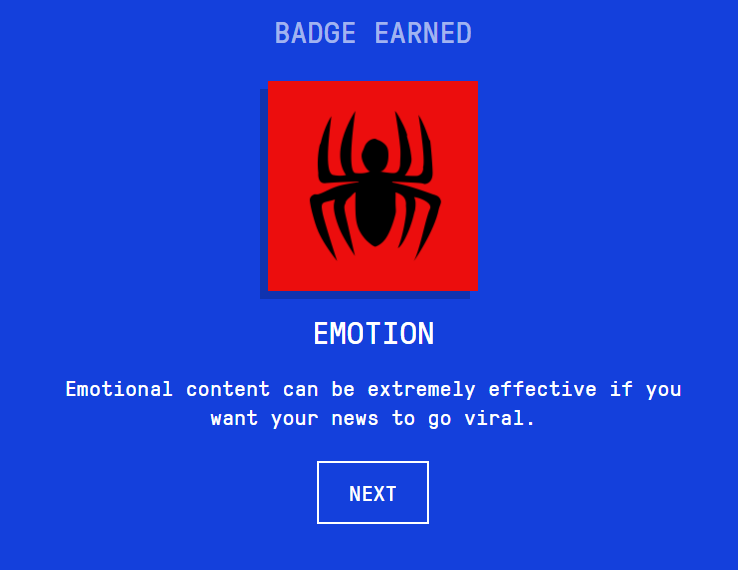
\includegraphics[trim=0 0 0 0, clip, width=\textwidth] {Capture2.PNG}
    \caption{Badge2}
    \label{fig2}
\end{figure}
\clearpage
\begin{figure}[h]
    \centering
    % trim and clip are used to crop the image, trim=left bottom right top
    % width sets max width, height will be scaled appropriately
    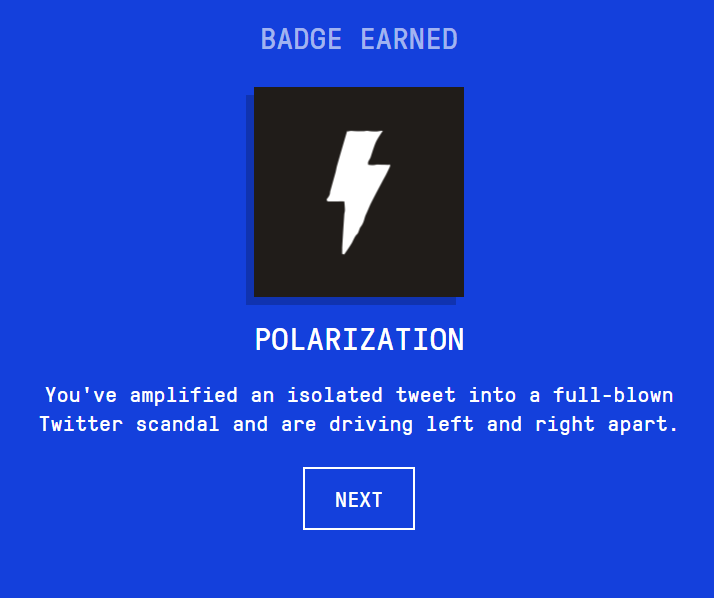
\includegraphics[trim=0 0 0 0, clip, width=\textwidth] {Capture3.PNG}
    \caption{Badge3}
    \label{fig3}
\end{figure}
\clearpage
\begin{figure}[h]
    \centering
    % trim and clip are used to crop the image, trim=left bottom right top
    % width sets max width, height will be scaled appropriately
    
\includegraphics[trim=0 0 0 0, clip, width=\textwidth] {Capture4.PNG}
    \caption{Badge4}
    \label{fig4}
\end{figure}
\clearpage
\begin{figure}[h]
    \centering
    % trim and clip are used to crop the image, trim=left bottom right top
    % width sets max width, height will be scaled appropriately
    
\includegraphics[trim=0 0 0 0, clip, width=\textwidth] {Capture5.PNG}
    \caption{Badge5}
    \label{fig5}
\end{figure}
\clearpage
\begin{figure}[h]
    \centering
    % trim and clip are used to crop the image, trim=left bottom right top
    % width sets max width, height will be scaled appropriately
    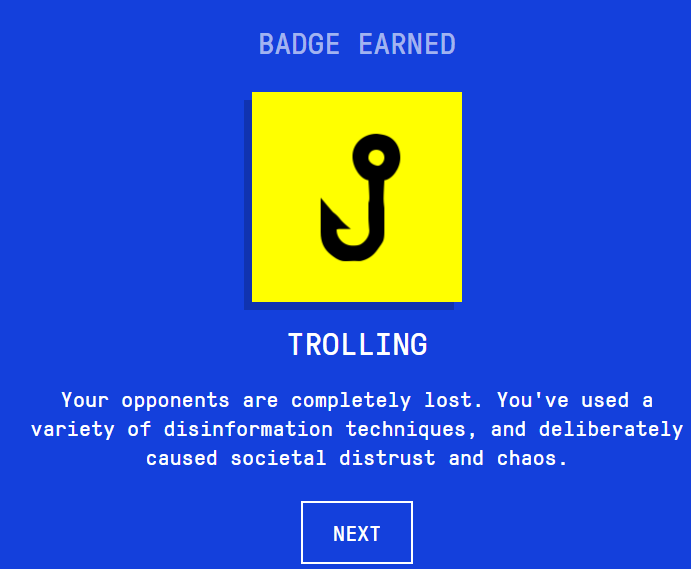
\includegraphics[trim=0 0 0 0, clip, width=\textwidth] {Capture6.PNG}
    \caption{Badge6}
    \label{fig6}
\end{figure}
\clearpage
\begin{figure}[h]
    \centering
    % trim and clip are used to crop the image, trim=left bottom right top
    % width sets max width, height will be scaled appropriately
    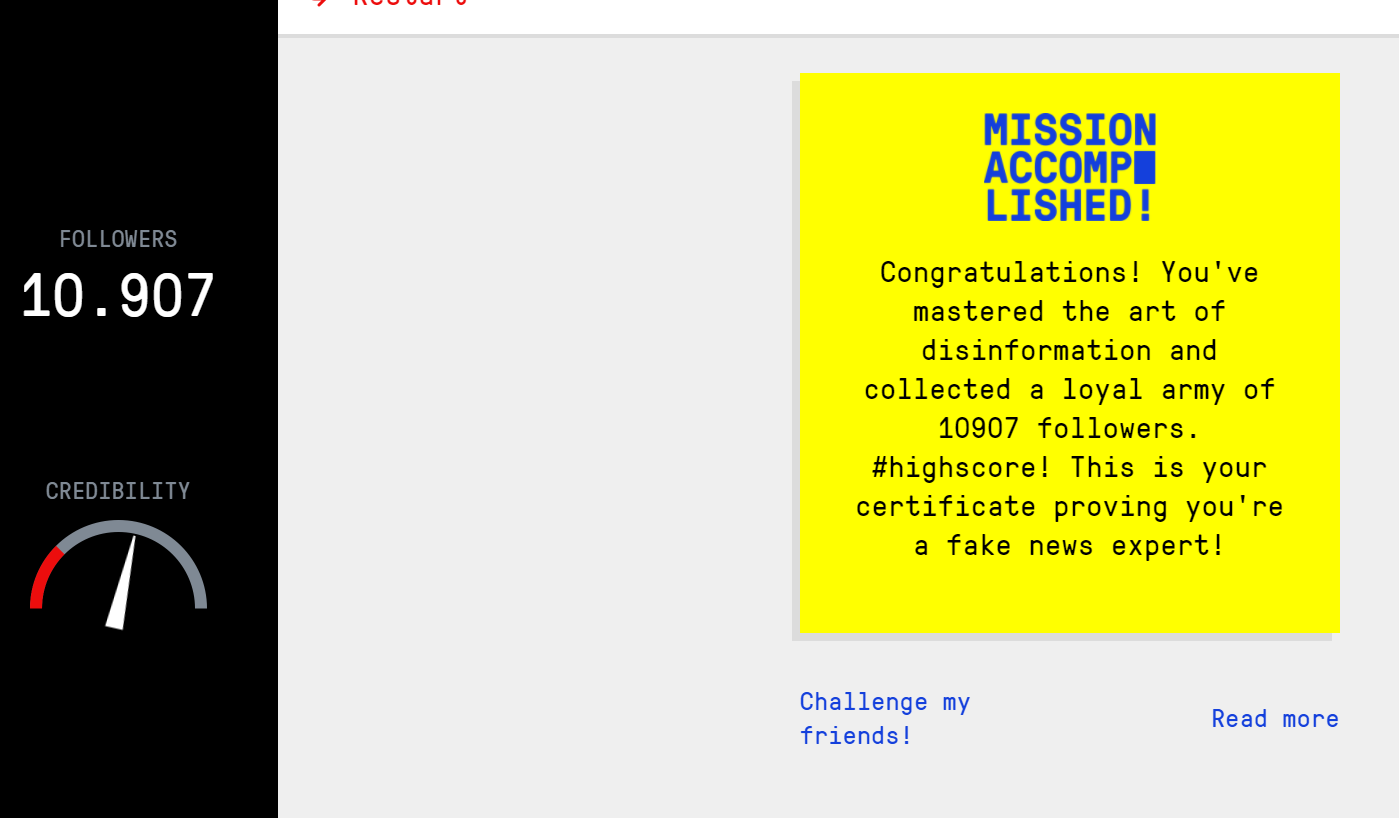
\includegraphics[trim=0 0 0 0, clip, width=\textwidth] {Capture7.PNG}
    \caption{Final Badge}
    \label{fig7}
\end{figure}
\subsection*{Discussion}
\emph{I used https://www.getbadnews.com/ to play the came and was able to earn the above badges below:}
\begin{itemize}
\item Impersonation in Figure \ref{fig1} (Impersonating someone else and disguising myself as a credible news source which was highly effective in increase my followers)
\item Emotion in Figure \ref{fig2} (Playing to people's emotion out of fear, anger or compassing was a great tool for spreading my messages)
\item Polarization in Figure \ref{fig3} (By finding existing grievance and blowing them out of proportion, drove people apart and made think a story is much more important that it really was.)
\item Conspiracy in Figure \ref{fig4}(I can use people's desires for the 'truth' as a tool to lure them into my band of followers)
\item Discredit in Figure \ref{fig5}(When someone is attacking my credibility i strike back. I do not apologize nor do I play nice and above all I do not retreat)
\item Trolling in Figure \ref{fig6} ( Is a tool that evokes an emotional response such as anger, irritation or sadness.)
\item The final score was 10907 followers in Figure \ref{fig7}.
\end{itemize}

\section*{References}
\begin{itemize}
\item {\url{https://www.datacamp.com/community/tutorials/pandas-read-csv}}
\item {\url{https://stackoverflow.com/questions/45164537/filter-pandas-data-frame-based-on-exact-string-match}}
\item {\url{https://pandas.pydata.org/docs/reference/api/pandas.DataFrame.sort_values.html}}
\item {\url{https://stackoverflow.com/questions/12021754/how-to-slice-a-pandas-data-frame-by-position}}
\item {\url{https://pandas.pydata.org/pandas-docs/stable/reference/api/pandas.DataFrame.rename.html}}
\item {\url{https://pandas.pydata.org/docs/reference/api/pandas.DataFrame.drop.html}}
\item {\url{https://stackoverflow.com/questions/38288372/unable-to-drop-a-column-from-pandas-dataframe}}
\item {\url{https://stackoverflow.com/questions/45164537/filter-pandas-data-frame-based-on-exact-string-match}}
\item {\url{https://stackoverflow.com/questions/39092067/pandas-dataframe-convert-column-type-to-string-or-categorical}}

\end{itemize}

\end{document}
\end{document}
\end{document}
